\chapter{矩阵之前}

    \section{补充:线性方程组}

        \subsection{唯一解,无解,无穷解问题}

            \begin{example}
                已知线性方程组$\begin{cases}3x_1+2x_2-x_3=6\\x_1+ax_2+2x_3=9\\2x_1-x_2+3x_3=3\end{cases}$有唯一解,则$a$应满足什么条件?
            \end{example}

            \begin{solution}
                \[
                    \begin{bmatrix}3&2&-1&6\\1&a&2&9\\2&-1&3&3\end{bmatrix}\rightarrow\begin{bmatrix}3&2&-1&6\\7&a+4&0&21\\11&5&0&21\end{bmatrix}\rightarrow\begin{bmatrix}3&2&-1&6\\0&a+\frac{9}{11}&0&*\\11&5&0&21\end{bmatrix}
                \]
                因此有唯一解的条件是$a\neq-\dfrac{9}{11}$。
            \end{solution}

            \begin{example}
                已知线性方程组$\begin{cases}\lambda x_1+x_2+x_3=1\\x_1+\lambda x_2+x_3=\lambda\\x_1+x_2+\lambda x_3=\lambda^2\end{cases}$有无穷多解,则$\lambda$应满足什么条件?
            \end{example}

            \begin{solution}
                \[
                    \begin{bmatrix}\lambda&1&1&1\\1&\lambda&1&\lambda\\1&1&\lambda&\lambda^2\end{bmatrix}\rightarrow\begin{bmatrix}0&1-\lambda&1-\lambda^2&1-\lambda^3\\0&\lambda-1&1-\lambda&\lambda-\lambda^2\\1&1&\lambda&\lambda^2\end{bmatrix}\rightarrow\begin{bmatrix}0&0&2-\lambda-\lambda^2&1+\lambda-\lambda^2-\lambda^3\\0&\lambda-1&1-\lambda&\lambda-\lambda^2\\1&1&\lambda&\lambda^2\end{bmatrix}
                \]
                因此有无穷多解的条件是$\begin{cases}2-\lambda-\lambda^2=0\\1+\lambda-\lambda^2-\lambda^3=0\end{cases}$,即$\lambda=1$.
            \end{solution}

        \subsection{插值问题}

            \begin{example}[(Lagrange插值)]
                求三次多项式$f(x)=ax^3+bx^2+cx+d$经过$(1,2),(-1,3),(3,0),(0,2)$.
            \end{example}

            \begin{solution}
                \[
                    \text{由题意有:}\begin{cases}a+b+c+d=2\\-a+b-c+d=3\\27a+9b+3c+d=0\\d=2\end{cases}
                \]
                \begin{flalign*}
                    &\begin{bmatrix}1&1&1&1&2\\-1&1&-1&1&3\\27&9&3&1&0\\0&0&0&1&2\end{bmatrix}\rightarrow\begin{bmatrix}1&1&1&0&0\\-1&1&-1&0&1\\27&9&3&0&-2\\0&0&0&1&2\end{bmatrix}\rightarrow\begin{bmatrix}1&1&1&0&0\\0&2&0&0&1\\0&-18&-24&0&-2\\0&0&0&1&2\end{bmatrix} \\
                    \rightarrow&\begin{bmatrix}1&1&1&0&0\\0&1&0&0&\frac12\\0&0&-24&0&7\\0&0&0&1&2\end{bmatrix}\rightarrow\begin{bmatrix}1&0&0&0&-\frac{5}{24}\\0&1&0&0&\frac12\\0&0&1&0&-\frac{7}{24}\\0&0&0&1&2\end{bmatrix}
                \end{flalign*}
                因此$a=-\dfrac{5}{24},b=\dfrac12,c=-\dfrac{7}{24},d=2$,$f(x)=-\dfrac{5}{24}x^3+\dfrac12x^2-\dfrac{7}{24}x+2$.
            \end{solution}

            $ $

            \begin{example}[(Hermite插值)]
                求三次多项式$f(x)=ax^3+bx^2+cx+d$满足$f(0)=2,f'(0)=2,f(1)=3,f'(1)=1$。
            \end{example}

            \begin{solution}
                易得$f'(x)=3ax^2+2bx+c$.
                \begin{flalign*}
                    &\begin{cases}d=2\\c=2\\a+b+c+d=3\\3a+2b+c=1\end{cases}\rightarrow\begin{bmatrix}0&0&0&1&2\\0&0&1&0&2\\1&1&1&1&3\\3&2&1&0&1\end{bmatrix}\rightarrow\begin{bmatrix}0&0&0&1&2\\0&0&1&0&2\\1&1&0&0&-1\\3&2&0&0&-1\end{bmatrix}\rightarrow\begin{bmatrix}0&0&0&1&2\\0&0&1&0&2\\1&1&0&0&-1\\0&-1&0&0&2\end{bmatrix} \qquad\qquad\qquad\qquad\\
                    \rightarrow&\begin{bmatrix}0&0&0&1&2\\0&0&1&0&2\\1&0&0&0&1\\0&1&0&0&-2\end{bmatrix}\rightarrow\begin{bmatrix}a\\b\\c\\d\end{bmatrix}=\begin{bmatrix}1\\-2\\2\\2\end{bmatrix}\qquad\Rightarrow\qquad f(x)=x^3-2x^2+2x+2
                \end{flalign*}
            \end{solution}

            \begin{example}
                求二次多项式$f(x)=ax^2+bx+c$满足$f(0)=2,f(1)=1,f'\left(\dfrac12\right)=2$.
            \end{example}

            \begin{solution}
                易得$f'(x)=2ax+b$.
                \begin{flalign*}
                    &\begin{cases}c=2\\a+b+c=1\\a+b=2\end{cases}\rightarrow\begin{bmatrix}0&0&1&2\\1&1&1&1\\1&1&0&2\end{bmatrix}\rightarrow\begin{bmatrix}0&0&1&2\\0&0&0&-3\\1&1&0&2\end{bmatrix}\quad\text{显然无解。}
                \end{flalign*}
            \end{solution}

            \begin{example}
                求三次多项式$f(x)=ax^3+bx^2+cx+d$满足$f(0)=2,f(1)=1,f'\left(\dfrac12\right)=2$。
            \end{example}

            \begin{solution}
                易得$f'(x)=3ax^2+2bx+c$.
                \begin{flalign*}
                    &\begin{cases}d=2\\a+b+c+d=1\\\frac34 a+b+c=2\end{cases}\rightarrow\begin{bmatrix}0&0&0&1&2\\1&1&1&1&1\\\frac34&1&1&0&2\end{bmatrix}\rightarrow\begin{bmatrix}0&0&0&1&2\\1&1&1&0&-1\\\frac34&1&1&0&2\end{bmatrix}\rightarrow\begin{bmatrix}0&0&0&1&2\\1&1&1&0&-1\\-\frac14&0&0&0&3\end{bmatrix}
                \end{flalign*}
                因此解为$\begin{bmatrix}a\\b\\c\\d\end{bmatrix}=\begin{bmatrix}-12\\-t+11\\t\\2\end{bmatrix}$,对应$f(x)=-12x^3+(-t+11)x^2+tx+2,\forall t\in\mathbb{R}$.
            \end{solution}

    \section{数与数域}

        \subsection{复数与单位根}

            \begin{theorem}[Euler]
                对于任意实数$\theta$,有$e^{i\theta}=\cos\theta+i\sin\theta$。特别地,当$\theta=\pi$时,有$e^{i\pi}+1=0$.
            \end{theorem}

            \begin{example}
                计算$\sum\limits_{j=0}^n\cos j\theta$和$\sum\limits_{j=0}^n\sin j\theta$.
            \end{example}

            \begin{solution}
                对$\theta =2k\pi$,有$\cos^{j}\theta = 1$,$\sin^{j}\theta = 0$,故$\sum\limits_{j=0}^n\cos j\theta = n+1$,$\sum\limits_{j=1}^n\sin j\theta = 0$.

                对$\theta \neq 2k\pi$,令$T=\sum\limits_{j=0}^{n}e^{ij\theta}=\sum\limits_{j=0}^n\cos j\theta+i\sum\limits_{j=0}^n\sin^{j}\theta$,有$e^{i\theta}T=T+e^{i(n+1)\theta}-1$,故$T=\dfrac{1-e^{i(n+1)\theta}}{1-e^{i\theta}}$.

                分别计算实部虚部,有$\sum\limits_{i=0}^n\cos i\theta = \dfrac{1-\cos(n+1)\theta}{2(1-\cos\theta)}$,$\sum\limits_{i=0}^n\sin i\theta = \dfrac{\sin (n+1)\theta-\sin \theta}{2(1-\cos\theta)}$.
            \end{solution}

            \begin{definition}
                $n$次单位根是指
                \begin{equation}
                    \label{eq:unit_root}
                    \cos\frac{2k\pi}n+i\sin\frac{2k\pi}n, k=0,1,\cdots,n-1
                    \nonumber
                \end{equation}
                这n个复数,记$\omega_n=\cos\dfrac{2\pi}n+isin\dfrac{2\pi}n$,则他们可以写为$\omega_n^{0},\omega_n^{1},\cdots,\omega_n^{n-1}$。
            \end{definition}

            之所以叫单位根,是因为其满足

            \begin{proposition}[单位根的性质]
                $n$次单位根是方程$x^n=1$的全部根.
            \end{proposition}

            根据\textbf{因式定理},可以推出

            \begin{equation}
                \label{eq:unit_root_factor}
                x^n-1=\prod_{k=0}^{n-1}(x-\omega_n^{k})
                \nonumber
            \end{equation}

            对比各项系数可以得到一些恒等式。事实上最常用的为:

            \begin{proposition}[单位根恒等式]
                \begin{enumerate}
                    \item
                        \begin{equation}
                            \label{eq:unit_root_identity1}
                            \sum_{k=0}^{n-1}(\omega_n^{k})^{m}=
                            \begin{cases}
                                n & n \mid m \\
                                0 & n \nmid m
                            \end{cases}
                            \nonumber
                        \end{equation}
                    \item
                        \begin{equation}
                            \label{eq:unit_root_identity2}
                            \omega_n^{a}=\omega_n^{a\pm n}
                            \nonumber
                        \end{equation}
                    \item
                        \begin{equation}
                            \label{eq:unit_root_identity3}
                            \overline{\omega_n^{a}}=\omega_n^{-a}
                            \nonumber
                        \end{equation}
                    \item
                        \begin{equation}
                            \label{eq:unit_root_identity4}
                            \omega_{mn}^{ma}=\omega_n^{a}
                            \nonumber
                        \end{equation}
                \end{enumerate}
            \end{proposition}

            \begin{proof}
                只证明(1).

                对$n\mid m,$有$\omega_n^{m}=1$,故$\sum\limits_{k=0}^{n-1}(\omega_n^{k})^{m}=\sum\limits_{k=0}^{n-1}1=n$.

                对$n\nmid m$,有$\omega_n^{m}\neq1$,故$\sum\limits_{k=0}^{n-1}(\omega_n^{k})^{m}=\sum\limits_{k=0}^{n-1}\omega_n^{km}=\dfrac{1-\omega_n^{nm}}{1-\omega_n^{m}}=0$.
            \end{proof}

            第二个恒等式就是最重要的\textbf{循环}性质。出于循环,它可以将一些东西按照模$n$的余数分类。

            \begin{example}
                计算$\sum\limits_{k=0}^{\lfloor \frac{n}{3} \rfloor}\dbinom{n}{3k}$,$\dbinom{n}{m}$为组合数$C_n^{m}$,$\lfloor x\rfloor$为向下取整,即不大于$x$的最大整数。
            \end{example}

            \begin{solution}
                考虑三次单位根$\omega_{3}=-\dfrac12+\dfrac{\sqrt{3}}{2}i$,由二项式定理有
                \begin{equation}
                    \label{eq:binomial_step1}
                    (1+1)^n=\sum_{k=0}^n\binom{n}{k}=\binom{n}{0}+\binom{n}{1}+\binom{n}{2}+\binom{n}{3}+\binom{n}{4}+\cdots
                \end{equation}
                \begin{equation}
                    \label{eq:binomial_step2}
                    (1+\omega_{3})^n=\sum_{k=0}^n\binom{n}{k}\omega_{3}^{k}=\binom{n}{0}+\binom{n}{1}\omega_{3}+\binom{n}{2}\omega_{3}^{2}+\binom{n}{3}+\binom{n}{4}\omega_{3}+\cdots
                \end{equation}
                \begin{equation}
                    \label{eq:binomial_step3}
                    (1+\omega_{3}^{2})^n=\sum_{k=0}^n\binom{n}{k}\omega_{3}^{2k}= \binom{n}{0}+\binom{n}{1}\omega_{3}^{2}+\binom{n}{2}\omega_{3}+\binom{n}{3}+\binom{n}{4}\omega_{3}^{2}+\cdots
                \end{equation}
                将(\ref{eq:binomial_step1}),(\ref{eq:binomial_step2})和(\ref{eq:binomial_step3})相加,注意到$1+\omega_{3}+\omega_{3}^{2}=0$,有
                \begin{equation}
                    \label{eq:binomial_step4}
                    (1+1)^n+(1+\omega_{3})^n+(1+\omega_{3}^{2})^n=3\sum_{k=0}^{\lfloor \frac{n}{3} \rfloor}\binom{n}{3k}
                    \nonumber
                \end{equation}
                即有
                \begin{equation}
                    \label{eq:binomial_step5}
                    \sum_{k=0}^{\lfloor \frac{n}{3} \rfloor}\binom{n}{3k}=\frac13(2^n+(1+\omega_{3})^n+(1+\omega_{3}^{2})^n)
                    \nonumber
                \end{equation}
            \end{solution}

            \begin{exercise}
                计算$\sum\limits_{k=0}^{\lfloor \frac{n-1}{3} \rfloor}\dbinom{n}{3k+1}$。
            \end{exercise}

            \begin{example}
                单位圆内接正n边形$A_{1}A_{2}A_{3}\dots A_n$中,$P$为单位圆上一点,证明:$\sum\limits_{k=1}^n|PA_{k}|^{2}=2n$。
            \end{example}

            \begin{proof}

                \begin{center}
                    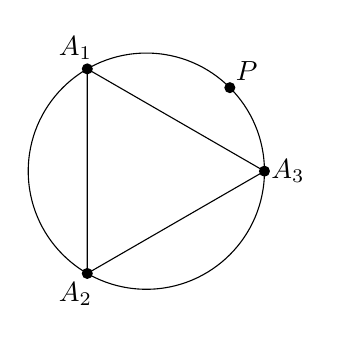
\begin{tikzpicture}
                        \draw (0,0) circle (1.5cm);
                        \coordinate (A1) at (120:1.5);
                        \coordinate (A2) at (240:1.5);
                        \coordinate (A3) at (0:1.5);
                        \coordinate (P) at (45:1.5);
                        \draw (A1) -- (A2) -- (A3) -- cycle;
                        \foreach \point in {A1, A2, A3, P}
                        \fill [black] (\point) circle (2pt);
                        \node at (120:1.8) {$A_1$};
                        \node at (240:1.8) {$A_2$};
                        \node at (0:1.8) {$A_3$};
                        \node at (45:1.8) {$P$};
                    \end{tikzpicture}
                \end{center}

                放在复平面上,设$A_{1}=\omega_n$,则$A_{k}=\omega_n^{k},\forall k=1,2,\cdots,n$。设$P=z$。

                \begin{equation}
                    \label{eq:unit_circle_proof1}
                    \Rightarrow\sum_{k=1}^n|PA_{k}|^{2}=\sum_{k=1}^n|z-\omega_n^{k}|^{2}=\sum_{k=1}^n(z-\omega_n^{k})(\overline{z}-\overline{\omega_n^{k}})=\sum_{k=1}^n\left( 1-\omega_n^{k}\overline{z}-z\overline{\omega_n^{k}}+1 \right)=2n
                    \nonumber
                \end{equation}

                最后一个等号用到$\sum\limits_{k=1}^n\omega_n^{k}=0$。
            \end{proof}

        \subsection{数环、数域}

            \begin{definition}[数环、数域]
                若复数域$\mathbb{C}$的某个包含1的子集$K$满足以下条件:
                \begin{enumerate}
                    \item $a,b\in K\Rightarrow a+b\in K$;
                    \item $a,b\in K\Rightarrow a-b\in K$;
                    \item $a,b\in K\Rightarrow ab\in K$;
                \end{enumerate}
                则称$K$为数环。

                若还满足$a\in K, a \neq 0\Rightarrow a^{-1}\in K$,则称$K$为数域。
            \end{definition}

            不难验证:

            \begin{proposition}[数环、数域-例子]
                有理数集$\mathbb{Q}$、实数集$\mathbb{R}$、复数集$\mathbb{C}$都是数域。整数集$\mathbb{Z}$是数环但不是数域。
            \end{proposition}

            \begin{note}
                当然,还有形态更复杂的数环和数域,例如所有$a+bi$在$a,b\in\mathbb{Z}$时构成数环,$a,b\in\mathbb{Q}$构成数域。
            \end{note}

            对于究竟怎样的集合是数环/数域,有一个简单的结论:

            \begin{proposition}[最小的数环、数域]
                任何数环包含$\mathbb{Z}$,任何数域包含$\mathbb{Q}$。
            \end{proposition}

    \section{杂项}

        \subsection{求和符号练习}

        线性代数中求和符号是一个重要的工具,有时候可以用来简化问题,有时候可以用来构造问题。在中学时,我们知道$\sum\limits_{i=1}^{n}a_i=a_1+a_2+\cdots+a_n$,除此之外,还有多重求和及集合求和。以下给出定义:

        \begin{definition}[多重求和及集合求和]
            (1)(多重求和)$\sum\limits_{a_1,a_2,\cdots,a_m=1}^{n}x_{a_{1}a_{2}\cdots a_{m}}\triangleq \sum\limits_{a_1,a_2,\cdots,a_{m-1}=1}^{n}x_{a_{1}a_{2}\cdots a_{m}}\sum\limits_{a_n=1}^n=\cdots=\sum\limits_{a_1=1}^n\sum\limits_{a_2=1}^n\cdots\sum\limits_{a_m=1}^{n}x_{a_{1}a_{2}\cdots a_{m}}$

            (2)(集合求和)$\sum\limits_{e\in\Lambda}x_e$用于表示对集合$\Lambda$中所有元素$e$的$x_e$值求和。集合$\Lambda$是索引集合,可以是有限的或无限的。索引集合包含所有我们想要求和的索引$e$。对于集合$\Lambda$中的每个元素$e$,$x_e$表示与$e$相关联的数值。$\sum$表示对所有$x_e$进行累加,其中$e$遍历集合$\Lambda$的所有元素。例如$\sum\limits_{i=1}^{n}a_i=\sum\limits_{e\in \{1,2,\cdots,n\}}a_e$。

            集合$\Lambda$也可以被替换为某一条件,例如$\sum\limits_{i=1}^{n}a_i=\sum\limits_{1\leq i\leq n}a_i,\sum\limits_{1\leq i<j\leq n}a_{ij}=\sum\limits_{i=1}^n\sum\limits_{j=i+1}^{n}a_{ij}$
        \end{definition}

        下面是一些求和符号的练习。

        \begin{example}
            证明:$\sum\limits_{i=1}^n\sum\limits_{j=1}^{m}a_{i}{b_j}=\sum\limits_{j=1}^{m}\sum\limits_{i=1}^{n}a_{i}{b_j}=\left(\sum\limits_{i=1}^{n}a_{i}\right) \left(\sum\limits_{j=1}^{m}b_{j}\right)$
        \end{example}

        \begin{proof}
            显然矩阵
            $\begin{bmatrix}
                a_{1}b_{1} & a_{1}b_{2} & \cdots & a_{1}b_{m} \\
                a_{2}b_{1} & a_{2}b_{2} & \cdots & a_{2}b_{m} \\
                \vdots & \vdots & \ddots & \vdots \\
                a_{n}b_{1} & a_{n}b_{2} & \cdots & a_{n}b_{m}
            \end{bmatrix}$
           的元素按行求和等于按列求和,故得证。
        \end{proof}

        \begin{example}
            计算$\sum\limits_{i=1}^n\sum\limits_{j=1}^n(i+j)^{2}$
        \end{example}

        \begin{solution}
            \begin{equation*}
                \begin{split}
                    \sum\limits_{i=1}^n\sum\limits_{j=1}^n(i+j)^{2}&=\sum\limits_{i=1}^n\sum\limits_{j=1}^n(i^{2}+j^{2}+2ij)=n\sum\limits_{i=1}^{n}i^{2}+\sum\limits_{j=1}^{n}j^{2}+2\sum\limits_{i=1}^n\sum\limits_{j=1}^{n}ij=2n\cdot\dfrac{n(n+1)(2n+1)}6+2\left(\sum\limits_{i=1}^{n}i\right)\left(\sum\limits_{j=1}^{n}j\right) \\
                                                                       &=\dfrac{n^2(n+1)(2n+1)}3+2\left(\dfrac{n(n+1)}2\right)^{2}=\dfrac{n^2(n+1)(7n+5)}6
                \end{split}
            \end{equation*}
        \end{solution}

        \begin{example}[(Chebyshev)]
            若$a_{1}\leq a_{2}\leq\cdots\leq a_n,b_{1}\leq b_{2}\leq\cdots\leq b_n$,则$\left(\sum\limits_{i=1}^{n}a_{i}\right)\left(\sum\limits_{j=1}^{n}b_{j}\right)\leq n\sum\limits_{k=1}^{n}a_{k}b_{k}$。
        \end{example}

        \begin{proof}
            只需证明$n\sum\limits_{k=1}^{n}a_{k}b_{k}-\left(\sum\limits_{i=1}^{n}a_{i}\right)\left(\sum\limits_{j=1}^{n}b_{j}\right)=\sum\limits_{1\leq j<i\leq n}(a_{i}-a_{j})(b_{i}-b_{j})\geq 0$。令$S=\sum\limits_{1\leq j<i\leq n}(a_{i}-a_{j})(b_{i}-b_{j})$.
            \begin{equation*}
                \begin{split}
                    2S&=\sum_{1\leq j<i\leq n}(a_{i}-a_{j})(b_{i}-b_{j})+\sum_{1\leq i<j\leq n}(a_{j}-a_{i})(b_{j}-b_{i})=\sum_{i,j=1}^n(a_{j}-a_{i})(b_{j}-b_{i}) \\
                      &=\sum_{i,j=1}^n(a_{j}b_{j}+a_{i}b_{i}-a_{i}b_{j}-a_{j}b_{i})=2n\sum_{k=1}^{n}a_{k}b_{k}-2\sum_{i,j=1}^{n}a_{i}b_{j}=2\left(n\sum_{k=1}^{n}a_{k}b_{k}-\left(\sum\limits_{i=1}^{n}a_{i}\right)\left(\sum\limits_{j=1}^{n}b_{j}\right)\right)
                \end{split}
            \end{equation*}
        \end{proof}

        \begin{example}
            记$H_{k}=\sum\limits_{j=1}^{k}\dfrac1j$,(1)求$\sum\limits_{1\leq j<k\leq n}\dfrac1{k-j}$(用$H_{k}$表示),(2)证明$\sum\limits_{j=1}^{n-1}H_{j}=nH_n-n$。
        \end{example}

        \begin{solution}
            $ $

            (1)$\sum\limits_{1\leq j<k\leq n}\dfrac1{k-j}=\sum\limits_{k=2}^n\sum\limits_{j=1}^{k-1}\dfrac1{k-j}=\sum\limits_{k=2}^n\sum\limits_{j=1}^{k-1}\dfrac1j=\sum\limits_{k=2}^{n}H_{k-1}=\sum\limits_{k=1}^{n-1}H_{k}$

            (2)$\sum\limits_{j=1}^{n-1}H_{j}=\sum\limits_{j=1}^{n-1}\sum\limits_{l=1}^{j}\dfrac1l=\sum\limits_{l=1}^{n-1}\sum\limits_{j=l}^{n-1}\dfrac1l=\sum\limits_{l=1}^{n-1}\dfrac{n-l}l=\sum\limits_{l=1}^n\dfrac{n-l}l=\sum\limits_{l=1}^n\left(\dfrac{n}l-1\right)=nH_n-n$
        \end{solution}

        \begin{example}[(Abel)]
            记$B_n=\sum\limits_{i=1}^{n}b_i$,则$S=\sum\limits_{i=1}^{n}a_{i}b_i=B_{n}a_n-\sum\limits_{i=1}^{n-1}B_i(a_{i+1}-a_i)$。
        \end{example}

        \begin{proof}
            \begin{equation*}
                \begin{split}
                    \sum_{i=1}^{n}a_{i}b_i&=\sum_{i=1}^{n}a_{i}(B_i-B_{i-1})=\sum_{i=1}^{n}a_{i}B_{i}-\sum_{i=1}^{n}a_{i}B_{i-1}=a_{n}B_{n}+\sum_{i=1}^{n-1}a_{i}B_{i}-\sum_{i=0}^{n-1}a_{i+1}B_i \\
                                          &=a_{n}B_{n}+\sum_{i=1}^{n-1}(a_{i}-a_{i+1})B_i-a_{1}B_{0}=B_{n}a_n-\sum_{i=1}^{n-1}B_i(a_{i+1}-a_i)
                \end{split}
            \end{equation*}
        \end{proof}

    \subsection{组合恒等式}

        \begin{lemma}
            \label{lemma:combinatorial_identity}
            \begin{enumerate}
                \item
                    \begin{equation*}
                        \binom{n}{k}=\binom{n}{n-k}(0\leq k\leq n)
                    \end{equation*}
                \item
                    \begin{equation*}
                        k\binom{n}{k}=n\binom{n-1}{k-1}
                    \end{equation*}
                \item
                    \begin{equation*}
                        \binom{n}{m}+\binom{n}{m+1}=\binom{n+1}{m+1}
                    \end{equation*}
            \end{enumerate}
        \end{lemma}

        \begin{theorem}[二项式定理]
            对$\forall x\in \mathbb{R}$及$n\in \mathbb{N}^*$,有$(1+x)^n=\sum\limits_{k=0}^{n}\dbinom{n}{k}x^{k}$。
        \end{theorem}

        \begin{proof}
            归纳。利用引理\ref{lemma:combinatorial_identity}\textbf{(3)},有
            \begin{equation*}
                (1+x)^n=(1+x)\cdot(1+x)^{n-1}=(1+x)\sum_{k=0}^{n-1}\binom{n-1}{k}x^{k}=\sum_{k=1}^{n-1}\left(\binom{n-1}{k-1}+\binom{n-1}{k}\right)x^{k}+1+x^n=\sum_{k=0}^{n}\binom{n}{k}x^{k}
            \end{equation*}
        \end{proof}

        \begin{corollary}
            利用上述定理和引理,可以得到:
            \begin{enumerate}
                \item
                    \begin{equation*}
                        \sum_{k=0}^{n}\binom{n}{k}=2^{n}
                    \end{equation*}
                \item
                    \begin{equation*}
                        \sum_{\substack{0\leq k\leq n \\ k\text{为偶数}}}\binom{n}{k}=\sum_{\substack{0\leq k\leq n \\ k\text{为奇数}}}\binom{n}{k}=2^{n-1}
                    \end{equation*}
                \item
                    \begin{equation*}
                        \binom{m+n}{k}=\sum_{i=0}^{k}\binom{m}{i}\binom{n}{k-i}\text{。特别地,}\binom{2n}{n}=\sum_{i=0}^{n}\binom{n}{i}^{2}
                    \end{equation*}
                \item
                    \begin{equation*}
                        \sum_{k=0}^{n}k\binom{n}{k}=n2^{n-1}
                    \end{equation*}
                \item
                    \begin{equation*}
                        \sum_{k=m}^{n}\binom{k}{m}=\binom{n+1}{m+1}
                    \end{equation*}
                \item
                    \begin{equation*}
                        \sum_{k=0}^{n}\binom{m+k}{k}=\binom{m+n+1}{n}
                    \end{equation*}
            \end{enumerate}
        \end{corollary}

        \begin{proof}
            (1)(2)对$(1+x)^n$使用二项式定理,分别取$x=1$和$x=-1$即可。

            (3)注意到$(1+x)^{m+n}=(1+x)^n\cdot(1+x)^m$,分别使用二项式定理,展开后比较$x^{k}$系数。

            (4)$(1+x)^n=\sum\limits_{k=0}^{n}\dbinom{n}{k}x^{k}$两侧对$x$求导,并取$x=1$即可。

            (5)
            \begin{equation}
                \label{eq:binomial_step6}
                \binom{k}{m}=const\left(\frac{(1+x)^k}{x^m}\right),\text{其中}const(f(x))\text{表示}f(x)\text{的常数项}
                \nonumber
            \end{equation}
            \begin{equation}
                \label{eq:binomial_step7}
                \Rightarrow \sum_{k=m}^n\binom{k}{m}=const\left(\sum_{k=m}^n\frac{(1+x)^k}{x^m}\right)=const\left(\frac1{x^{m}}\frac{(1+x)^{n+1}-(1+x)^{m}}{x}\right)=const\left(\frac{(1+x)^{n+1}}{x^{m+1}}\right)=\binom{n+1}{m+1}.
                \nonumber
            \end{equation}

            (6)利用引理\ref{lemma:combinatorial_identity}\textbf{(3)}归纳即可。
        \end{proof}

        \begin{example}
            设$n\leq m$,证明:$\sum\limits_{k=0}^{m}\dbinom{m}{k}\dbinom{n+k}{m}=\sum\limits_{k=0}^{m}\dbinom{m}{k}\dbinom{n}{k}2^k$。
        \end{example}

        \begin{proof}
            \begin{equation*}
                \begin{split}
                    \sum\limits_{k=0}^{m}\dbinom{m}{k}\dbinom{n+k}{m}&=[x^m](1+x)^n\sum_{k=0}^m\binom{m}{k}(1+x)^k=[x^m](1+x)^{n}(2+x)^m \\
                                                                     &=[x^m](1+x)^n\sum_{k=0}^m\binom{m}{k}2^{k}x^{m-k}=\sum_{k=0}^{m}\dbinom{m}{k}\dbinom{n}{k}2^k
                \end{split}
            \end{equation*}
            其中$[x^m]f(x)$表示多项式$f(x)$的$m$次项系数。
        \end{proof}
